% This LaTeX was auto-generated from MATLAB code.
% To make changes, update the MATLAB code and export to LaTeX again.

\documentclass{article}

\usepackage[utf8]{inputenc}
\usepackage[T1]{fontenc}
\usepackage{lmodern}
\usepackage{graphicx}
\usepackage{color}
\usepackage{listings}
\usepackage{hyperref}
\usepackage{amsmath}
\usepackage{amsfonts}
\usepackage{epstopdf}
\usepackage{matlab}

\sloppy
\epstopdfsetup{outdir=./}
\graphicspath{ {./ejercicio09_images/} }

\matlabmultipletitles

\begin{document}

\matlabtitle{Ejercicio Nº9}


\begin{matlabcode}
clear;clc;
\end{matlabcode}

\matlabtitle{Respuesta al impulso}

\begin{matlabcode}
syms C1 C2 C3 C4 C5 s R1 R2 R3 R4 R5 E1 v1 v2 v3 v4 v5;
\end{matlabcode}

\begin{par}
\begin{flushleft}
La matriz de admitancias
\end{flushleft}
\end{par}

\begin{matlabcode}
Y=[1/R1+s*C1+1/R2 -1/R2 0 0 0; -1/R2 1/R2+s*C2+1/R3 -1/R3 0 0;0 -1/R3 1/R3+s*C3+1/R4 -1/R4 0; 0 0 -1/R4 1/R4+s*C4+1/R5 -1/R5; 0 0 0 -1/R5 1/R5+s*C5]
\end{matlabcode}
\begin{matlabsymbolicoutput}
Y = 
    $\displaystyle \left(\begin{array}{ccccc}
C_1  s+\frac{1}{R_1 }+\frac{1}{R_2 } & -\frac{1}{R_2 } & 0 & 0 & 0\\
-\frac{1}{R_2 } & C_2  s+\frac{1}{R_2 }+\frac{1}{R_3 } & -\frac{1}{R_3 } & 0 & 0\\
0 & -\frac{1}{R_3 } & C_3  s+\frac{1}{R_3 }+\frac{1}{R_4 } & -\frac{1}{R_4 } & 0\\
0 & 0 & -\frac{1}{R_4 } & C_4  s+\frac{1}{R_4 }+\frac{1}{R_5 } & -\frac{1}{R_5 }\\
0 & 0 & 0 & -\frac{1}{R_5 } & C_5  s+\frac{1}{R_5 }
\end{array}\right)$
\end{matlabsymbolicoutput}
\begin{matlabcode}
Is=[E1/R1;0;0;0;0];
x=[v1;v2;v3;v4;v5];
Y\(Is)==x;
eqs=Y*x==Is;
solu=solve(eqs);
\end{matlabcode}


\begin{par}
\begin{flushleft}
Reemplazando los valores del circuito
\end{flushleft}
\end{par}

\begin{matlabcode}
C1=0.1;C2=0.1;C3=0.1;C4=0.1;C5=0.1;R1=1;R2=1;R3=1;R4=1;R5=1;E1=1;
\end{matlabcode}

\begin{par}
\begin{flushleft}
La función de transferencia $ H(s)=V5(s)/E(s)$
\end{flushleft}
\end{par}

\begin{matlabcode}
v5s=subs(solu.v5)
\end{matlabcode}
\begin{matlabsymbolicoutput}
v5s = 
    $\displaystyle \frac{1}{\frac{s^5 }{100000}+\frac{9 s^4 }{10000}+\frac{7 s^3 }{250}+\frac{7 s^2 }{20}+\frac{3 s}{2}+1}$
\end{matlabsymbolicoutput}
\begin{matlabcode}
v5t=vpa(rewrite(ilaplace(v5s),'exp'),4)
\end{matlabcode}
\begin{matlabsymbolicoutput}
v5t = 
    $\displaystyle 2.72 e^{-17.15 t} +0.5539 e^{-36.83 t} +1.014 e^{-0.8101 t} -2.5 e^{-6.903 t} -1.788 e^{-28.31 t} $
\end{matlabsymbolicoutput}


\matlabtitle{Respuesta al pulso con método Backward Euler}

\begin{matlabcode}
vc1=0;vc2=0;vc3=0;vc4=0;vc5=0;
Xant=[vc1;vc2;vc3;vc4;vc5];
ti=0;
tf=10;
h=0.01;
M=[C1 0 0 0 0; 0 C2 0 0 0; 0 0 C3 0 0; 0 0 0 C4 0; 0 0 0 0 C5];
N=[1/R1+1/R2 -1/R2 0 0 0; -1/R2 1/R2+1/R3 -1/R3 0 0; 0 -1/R3 1/R3+1/R4 -1/R4 0; 0 0 -1/R4 1/R4+1/R5 -1/R5; 0 0 0 -1/R5 1/R5];
solu=[];
it=1;
for i= ti:h:tf
    %Fuente variable
    if i<1
        E(it,1)=1;
    else
        E(it,1)=0;
    end

    %Se calcula el valor de la matriz u para cada punto 
    u=[E(it,1)/R1;0;0;0;0];
    
    X=((((1/h).*M)+N)\u) + ((((1/h).*M)+N)\((1/h).*M)*Xant);
    
    solu=[solu X];
    Xant=X;
    it=it+1;
end
t=ti:h:tf;
clf;
plot(t,solu(5,:),'--b')
hold on
fplot(v5t,[0,10],'-b')
ylim([0,0.7])
grid;
legend({'Rta. Pulso','Rta. Impulso'})
title('Respuesta temporal VC5(t)')
xlabel('tiempo [s]')
ylabel('Voltaje [V]')
\end{matlabcode}
\begin{center}
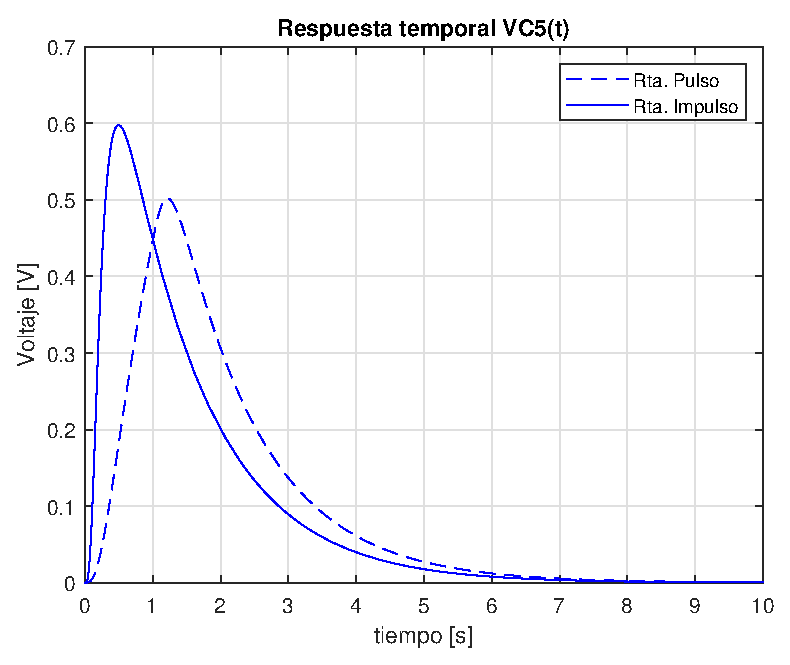
\includegraphics[width=\maxwidth{56.196688409433015em}]{figure_0_09}
\end{center}

\end{document}
